\section{Tasks}
\label{sec:module.Tasks}

\begin{figure}[bth]
\centering
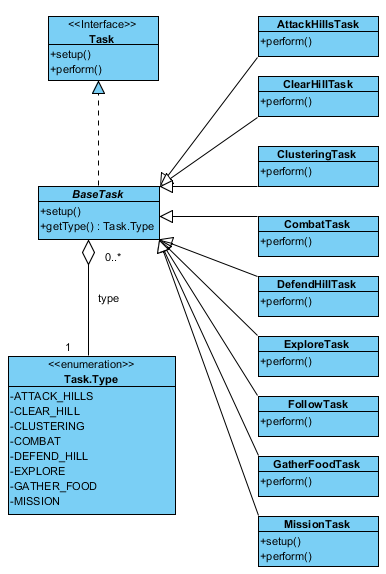
\includegraphics[width=0.5\textwidth]{91_bilder/Tasks}
\caption{Tasks}
\label{fig:tasks}
\end{figure}
Zu Beginn des Projekts haben wir die wichtigsten Aufgaben einer Ameise identifiziert. Diese Aufgaben wurden als Tasks in eigenen Klassen implementiert. Das Interface Task\footnote{Das Interface ist im Code unter ants.tasks.Bot.Java auffindbar.} definiert eine setup()-Methode welche den Task initiiert, sowie eine perform()-Methode welche den Task ausf�hrt. Im Programm werden die Tasks nach deren Wichtigkeit ausgef�hrt, was auch der nachfolgenden Reihenfolge entspricht. Jedem Task stehen nur die unbesch�ftigten Ameisen zur Verf�gung, d.h. jene welchen noch keine Aufgabe zugeteilt wurde.

\subsubsection{MissionTask}
\label{subsec:implementation.Tasks.MissionTask}
Dieser Task pr�ft alle aktuellen Missionen auf deren G�ltigkeit, beispielsweise ob die Ameise der Mission den letzten Zug �berlebt hat und die Mission weiterf�hren kann. Falls g�ltig, wird der n�chste Schritt der Mission ausgef�hrt.

\subsubsection{GatherFoodTask}
\label{subsec:implementation.Tasks.GatherFoodTask}
F�r jedes Food-Tile werden in einem definierbaren Radius r die n�chsten Ameisen bestimmt. Danach wird nach aufsteigender Luftliniendistanz mit dem Pfadsuchalgorithmus SIMPLE (s. Abschnitt \ref{subsec:implementation.Pfadsuche.Simple}) oder -- falls dieser keinen Pfad gefunden hat -- mit A* eine passierbare Route gesucht. Wenn ein Pfad existiert, kann mit der Ameise und dem Food-Tile eine GatherFoodMission erstellt werden, welche die Ameise zum Food-Tile f�hrt. Zu jedem Food-Tile wird immer nur eine Ameise geschickt.

\subsubsection{AttackHillsTask}
\label{subsec:implementation.Tasks.AttackHillsTask}
Sobald gegnerische Ameisenhaufen sichtbar sind, sollen diese angegriffen werden. Das Zerst�ren eines gegnerischen Haufens ist wie erw�hnt 2 Punkte wert. Die Kriterien, nach denen eine Pfad zum gegnerischen Haufen gesucht wird, sind die selben wie beim GatherFoodTask, ausser dass mehrere Ameisen das Ziel angreifen k�nnen. Es wird eine AttackHillMission erstellt.

\subsubsection{CombatTask}
\label{subsec:implementation.Tasks.CombatTask}
Beim Angriffstask wird berechnet ob wir in einem Kampfgebiet (definiert �ber den Sichtradius einer Ameise) die �berhand, d.h. mehr Ameisen platziert haben. Falls ja, wird die gegnerische Ameise angegriffen.

\subsubsection{DefendAreaTask}
\label{subsec:implementation.Tasks.DefendAreaTask}
Dieser Task w�re vogesehen um eine Region wie zum Beispiel den eigenen Ameisenh�gel zu sch�tzen. Dieser Task wurde im Zuge dieser Arbeit nicht implementiert.

\subsubsection{ExploreTask}
\label{subsec:implementation.Tasks.ExploreTask}
F�r alle noch unbesch�ftigten Ameisen wird mittels ManhattanDistance der n�chste Ort gesucht, der noch nicht sichtbar, also unerforscht ist. Falls ein Pfad mittels Pfadsuchalgorithmus gefunden wird, wird eine ExploreMission (s. Abschnitt \ref{sec:implementation.Missionen}) erstellt. Die Ameise wird den gefundenen Pfad in den n�chsten Spielz�gen ablaufen.

\subsubsection{FollowTask}
\label{subsec:implementation.Tasks.FollowTask}
Der FollowTask ist f�r Ameisen angedacht welche aktuell keine Aufgabe haben. Diese Ameisen sollen einer nahe gelegenen, besch�ftigten Ameise folgen, damit diese nicht alleine unterwegs ist.

\subsubsection{ClearHillTask}
\label{subsec:implementation.Tasks.ClearHillTask}
Dieser Task bewegt alle Ameisen, welche neu aus unserem H�gel ''schl�pfen``, vom H�gel weg. So werden nachfolgende Ameisen nicht durch diese blockiert.

\subsubsection{ClusteringTask}
\label{subsec:implementation.Tasks.ClusteringTask}
Der ClusteringTask wird als Vorbereitung f�r den HPA* Algorithmus verwendet. Hier wird f�r alle sichtbaren Kartenregionen ein Clustering vorgenommen. Das Clustering wird im Kapitel \ref{subsec:implementation.Pfadsuche.HPAstar} im Detail beschreiben.
